\section*{ÔN TẬP CHƯƠNG IV}
\subsection{Bài tập tự luận}
%%==========Bài 1
\begin{bt}
	Tìm số đo góc $\alpha$ biết rằng
	\begin{listEX}[4]
	\item $\sin\alpha=0{,}25$;
	\item $\cos\alpha=0{,}75$;
	\item $\tan\alpha=1$;
	\item $\cot\alpha=2$.
	\end{listEX}
	\loigiai{
	\begin{listEX}[2]
	\item $\sin\alpha=0{,}25\Rightarrow \alpha \approx 14^\circ$;
	\item $\cos\alpha=0{,}75\Rightarrow \alpha \approx 41^\circ$;
	\item $\tan\alpha=1\Rightarrow \alpha = 45^\circ$;
	\item $\cot\alpha=2\Rightarrow \alpha \approx 27^\circ$.
	\end{listEX}
	}
\end{bt}
%%==========Bài 2
\begin{bt}
	\immini{Cho tam giác $A B C$ vuông tại $A$, có $\widehat{B}=\alpha$.
	\begin{enumerate}
	\item Hãy viết các tỉ số lượng giác $\sin \alpha, \cos \alpha$.
	\item Sử dụng định lí Pythagore, chứng minh rắng $\sin ^2 \alpha+\cos ^2 \alpha=1$.
	\end{enumerate}}{\begin{tikzpicture}[scale=0.75, font=\footnotesize, line join=round, line cap=round, >=stealth]
	\def\r{2}
	\path
	(0,0) coordinate (A)
	(0,3) coordinate (C)
	(-2,0) coordinate (B)
	;
	\draw
	($(B)+(0.4,0.2)$) node{$\alpha$}
	(A)--(B)--(C)--cycle
	pic[draw, angle radius=2mm]{right angle=B--A--C}
	pic[draw, angle radius=2mm]{angle=A--B--C};
	\foreach \x/\g in{A/-90, B/-90, C/0} \fill[black](\x) circle (1pt) ($(\x)+(\g:3mm)$) node{\x};
	\end{tikzpicture}}
	\loigiai{
	\begin{enumerate}
	\item $\sin \alpha = \dfrac{AC}{BC}$, $\cos\alpha =\dfrac{AB}{BC}$.
	\item Ta có $\sin^2\alpha = \dfrac{AC^2}{BC^2}$, $\cos^2\alpha =\dfrac{AB^2}{BC^2}$.\\
	Suy ra $\sin ^2 \alpha+\cos ^2 \alpha=\dfrac{AC^2}{BC^2}+\dfrac{AB^2}{BC^2}=\dfrac{AC^2+AB^2}{BC^2}=\dfrac{BC^2}{BC^2}=1.$ (Vì tam giác $ABC$ vuông tại $A$)
	\end{enumerate}
	}
\end{bt}
%%==========Bài 3
\begin{bt}%[MaT-SGK9-Moi]%[Quan Ón - Thầy Hải Toán]
	Cho tam giác $ABC$ vuông tại $A$ có đường cao $AH$ và $\widehat{B} = \alpha$ (hình bên dưới).
	\immini{
	\begin{enumerate}
	\item Tỉ số $\dfrac{HA}{HB}$ bằng
	\choice
	{$\sin \alpha$}
	{$\cos \alpha$}
	{$\tan \alpha$}
	{$\cot \alpha$}
	\item Tỉ số $\dfrac{HA}{HC}$ bằng
	\choice
	{$\sin \alpha$}
	{$\cos \alpha$}
	{$\tan \alpha$}
	{$\cot \alpha$}
	\item Tỉ số $\dfrac{HA}{AC}$ bằng
	\choice
	{$\sin \alpha$}
	{$\cos \alpha$}
	{$\tan \alpha$}
	{$\cot \alpha$}
	\end{enumerate}
	}{
	\begin{tikzpicture}[>=stealth,line join=round,line cap=round,font=\footnotesize,scale=1]
	\path 
	(1.61,2.12) coordinate (A)
	(0,0) coordinate (B)
	(4.41,0) coordinate (C)
	($(B)!(A)!(C)$) coordinate (H);
	\draw (A)--(B)--(C)--(A)--(H);
	\foreach \l/\g in {A/90,B/-135,C/-45,H/-90}
	\draw[fill=black] (\l) circle (1pt) +(\g:.3) node{$\l$};
	\pic[draw,angle radius=2mm,angle eccentricity=1.5] {right angle = A--H--C};
	\pic[draw,angle radius=2mm,angle eccentricity=1.5] {right angle = B--A--C};
	\pic[draw,angle radius=4mm,angle eccentricity=1.5] {angle = C--B--A};
	\draw (B) circle (1pt) +(22:.6) node[scale=1.1]{$\alpha$};
	\end{tikzpicture}
	}
	\loigiai{
	\begin{enumerate}
	\item Xét $\triangle HAB$ vuông tại $H$, ta có $\tan \alpha = \dfrac{HA}{HB}$.\\
	Đáp án: C. $\tan \alpha$.
	\item Xét $\triangle HAC$ vuông tại $H$, ta có $\tan (90^\circ - \alpha) = \dfrac{HA}{HC}$.\\
	Suy ra $\cot \alpha = \dfrac{HA}{HC}$.\\
	Đáp án: D. $\cot \alpha$.
	\item Xét $\triangle HAC$ vuông tại $H$, ta có $\sin(90^\circ - \alpha) = \dfrac{HA}{AC}$.\\
	Suy ra $\cos\alpha = \dfrac{HA}{AC}$.\\
	Đáp án: B. $\cos \alpha$.
	\end{enumerate}
	}
\end{bt}
%%==========Bài 4
\begin{bt}
	Cho tam giác $ABC$ vuông tại $A$ có $AB=18$ cm, $AC=24$ cm. Tính các tỉ số lượng giác của góc $B$, từ đó suy ra các tỉ số lượng giác của góc $C$.
	\loigiai{
	\immini{
	Áp dụng định lí Pi-ta-go ta có\\
	$BC^2=AB^2+AC^2=18^2+24^2=900\Rightarrow BC=\sqrt{900}=30 ~\mathrm{cm}.$
	\begin{itemize}
	\item $\sin B=\dfrac{AC}{BC}=\dfrac{24}{30}=\dfrac{4}{5}$.
	\item $\cos B=\dfrac{AB}{BC}=\dfrac{18}{30}=\dfrac{3}{5}$.
	\item $\tan B=\dfrac{AC}{AB}=\dfrac{24}{18}=\dfrac{4}{3}$.
	\item $\cot B=\dfrac{AB}{AC}=\dfrac{18}{24}=\dfrac{3}{4}$.
	\end{itemize}}{\begin{tikzpicture}[scale=1, font=\footnotesize, line join=round, line cap=round, >=stealth]
	\path
	(0,0) coordinate (A)
	(0,3) coordinate (B)
	(4,0) coordinate (C)
	;
	\draw 
	(A)--(B)node[midway,left]{$18$}--(C)--(A)node[midway,below]{$24$}
	;
	\foreach \p/\g in {A/200, B/150, C/0}
	\draw[fill=black] (\p) circle (1pt) node[shift=(\g:3mm)] {$\p$};
	\end{tikzpicture}}
	Suy ra $\sin C=\cos B=\dfrac{3}{5}$; $\cos C=\sin B=\dfrac{4}{5}$; $\tan C=\cot B=\dfrac{3}{4}$; $\cot C=\tan B=\dfrac{4}{3}$.
	}
\end{bt}
%%==========Bài 5
\begin{bt}
	Xét các tam giác vuông có một góc nhọn bằng hai lần góc nhọn còn lại. Hỏi các tam giác đó có đồng dạng với nhau không? Tính $\sin$ và côsin của góc nhọn lớn hơn.
	\loigiai{
	\immini{Xét tam giác $ABC$ có $\widehat{B}=2\widehat{C}$.
	\begin{itemize}
	\item Các tam giác này không đồng dạng với nhau vì các góc nhọn tương ứng có số đo không bằng nhau.
	\item Ta có $\sin B=\dfrac{AC}{BA}$, $\cos B=\dfrac{AB}{BC}$.
	\end{itemize}
	}{\begin{tikzpicture}[scale=0.8, font=\footnotesize, line join=round, line cap=round, >=stealth]
	\def\r{2}
	\path
	(0,0) coordinate (A)
	(0,3) coordinate (C)
	(-2,0) coordinate (B)
	;
	\draw
	($(B)+(0.55,0.2)$) node{$\alpha$}
	(A)--(B)--(C)--cycle
	;
	\foreach \x/\g in{A/-90, B/-90, C/0} \fill[black](\x) circle (1pt) ($(\x)+(\g:3mm)$) node{\x};
	\draw pic[draw, angle radius=3mm]{angle=A--B--C};
	\draw pic[draw=black,angle radius=5pt] {right angle = B--A--C};
	\end{tikzpicture}}
	}
\end{bt}
%%==========Bài 6
\begin{bt}
	Cho góc nhọn $\alpha$ biết $\sin \alpha=0{,}8$. Tính $\cos \alpha$, $\tan\alpha$, $\cot\alpha$.
	\loigiai{
	Ta có $\sin \alpha =0{,}8\Rightarrow \alpha\approx53^\circ$.\\
	Suy ra 
	\begin{enumEX}[\itemCI]{3}
	\item $\cos \alpha=\cos 53^\circ\approx0{,}6018$.
	\item $\tan\alpha=\tan 53^\circ\approx1{,}327$.
	\item $\cot\alpha=\cot 53^\circ\approx0{,}7536$.
	\end{enumEX}
	}
\end{bt}
%%==========Bài 7
\begin{bt}
	Tính giá trị của biểu thức
	\begin{enumerate}
	\item $A=4-\sin^2 45^\circ+2\cos^2 60^\circ-3\cot^2 45^\circ$;
	\item $B=\tan 45^\circ\cdot \cos 30^\circ\cdot\cot30^\circ$;
	\item $C=\sin 15^\circ+\sin 75^\circ-\cos 15^\circ-\cos 75^\circ+\sin 30^\circ$.
	\end{enumerate}
	\loigiai{
	\begin{enumerate}
	\item $A=4-\sin^2 45^\circ+2\cos^2 60^\circ-3\cot^2 45^\circ=4-\left(\dfrac{\sqrt{2}}{2}\right)^2+2\left(\dfrac{1}{2}\right)^2-3\cdot1^2=1$.
	\item $B=\tan 45^\circ\cdot \cos 30^\circ\cdot\cot30^\circ=1\cdot\dfrac{\sqrt{3}}{2}\cdot\sqrt{3}=\dfrac{3}{2}$.
	\item $\begin{aligned}[t]C&=\sin 15^\circ+\sin 75^\circ-\cos 15^\circ-\cos 75^\circ+\sin 30^\circ\\&=\cos75^\circ+\cos15^\circ-\cos 75^\circ+\sin 30^\circ\\&=\sin30^\circ=\dfrac{1}{2}.\end{aligned}$
	\end{enumerate}
	}
\end{bt}
%%==========Bài 8
\begin{bt}
	Cho tam giác $OPQ$ vuông tại $O$ có $\widehat{P}=39^\circ$ và $PQ=10$ cm. Hãy giải tam giác vuông $OPQ$.
	\loigiai{
	\immini{
	Ta có $\widehat{Q}=90^\circ-\widehat{P}=90^\circ-39^\circ=51^\circ$.\\
	Tam giác $PQO$ vuông tại $O$ nên
	\begin{itemize}
	\item $OQ=PQ\cdot\sin P=10\cdot\sin39^\circ\approx6{,}3$ cm.
	\item $OP=PQ\cdot\cos P=10\cdot\cos39^\circ\approx7{,}8$ cm.
	\end{itemize}
	}{\begin{tikzpicture}[scale=1, font=\footnotesize, line join=round, line cap=round, >=stealth]
	\def\r{2}
	\path
	(130:\r) coordinate (O)
	(180:\r) coordinate (P)
	(0:\r) coordinate (Q)
	;
	\draw
	(O)--(P)--(Q)node[midway,below]{$10$ cm}--cycle
	pic[draw, angle radius=2mm]{right angle=P--O--Q};
	\foreach \x/\g in{O/90, P/180, Q/0} \fill[black](\x) circle (1pt)
	($(\x)+(\g:3mm)$) node{$\x$};
	\pic["\tiny{$39^\circ$}",draw,angle radius=8mm]{angle=Q--P--O};
	\end{tikzpicture}}
	}
\end{bt}
%%==========Bài 9
\begin{bt}
	Cho tam giác $ABC$ vuông tại $A$. Chứng minh rằng $\dfrac{AC}{AB}=\dfrac{\sin B}{\sin C}$.
	\loigiai{
	\immini{
	Tam giác $ABC$ vuông tại $A$ nên ta có $$\sin B=\dfrac{AC}{BC};\, \sin C=\dfrac{AB}{BC}.$$
	Suy ra $\dfrac{\sin B}{\sin C}=\dfrac{AC}{BC}:\dfrac{AB}{BC}=\dfrac{AC}{AB}$.
	}{\begin{tikzpicture}[scale=1, font=\footnotesize, line join=round, line cap=round, >=stealth]
	\def\r{2}
	\path
	(130:\r) coordinate (A)
	(180:\r) coordinate (B)
	(0:\r) coordinate (C)
	;
	\draw
	(A)--(B)--(C)--cycle
	pic[draw, angle radius=2mm]{right angle=B--A--C};
	\foreach \x/\g in{A/90, B/180, C/0} \fill[black](\x) circle (1pt)
	($(\x)+(\g:3mm)$) node{\x};
	\end{tikzpicture}}
	}
\end{bt}
%%==========Bài 10
\begin{bt}%[MaT-SGK9-Moi]%[Thầy Hải Toán - Quan Ón]
	Cho hình thoi $ABCD$ có $AB=a$, $\widehat{BAD}=2\alpha\;\left(0^\circ<\alpha<90^\circ\right)$. Chứng minh:
	\begin{listEX}[2]
	\item $BD=2a\cdot\sin\alpha$;
	\item $AC=2a\cdot\cos\alpha$.
	\end{listEX}
	\loigiai
	{
	\begin{center}
	\begin{tikzpicture}[line join = round, line cap = round,>=stealth,font=\footnotesize,scale=1,declare function={ao=2;gocA=60;ab=ao/(cos(gocA/2));}]
	\path 
	(0,0) coordinate (O)
	(-ao,0) coordinate (A)
	($(A)+(gocA/2:ab)$) coordinate (B)
	(ao,0) coordinate (C)
	($(A)+(-gocA/2:ab)$) coordinate (D)
	;
	\draw (A)--(B)--(C)--(D)--cycle (A)--(C) (B)--(D);
	\foreach \x/\gm in {A/180,B/90,C/0,D/-90,O/-45} \fill (\x) circle (1pt) ($(\x)+(\gm:3.5mm)$)node{$\x$};
	\foreach \x/\y/\z in {B/O/A} \draw pic[draw,angle radius=2.5mm]{right angle=\x--\y--\z};
	\end{tikzpicture}
	\end{center}
	\begin{enumerate}
	\item Gọi $O$ là giao điểm của $AC$ và $BD$ suy ra $AO\perp OB$, $\widehat{BAO}=\dfrac{\widehat{BAD}}{2}=\alpha$.\\
	Trong tam giác vuông $ABO$ theo tỉ số lượng giác ta có \allowdisplaybreaks
	\begin{eqnarray*}
	&&\sin\widehat{BAO}=\dfrac{BO}{AB}\\
	&& BO=AB\cdot\sin\widehat{BAO}\\
	&& BO=AB\cdot\sin\alpha
	\end{eqnarray*}
	Suy ra $BD=2BO=2a\sin\alpha$.
	\item Trong tam giác vuông $ABO$ theo tỉ số lượng giác ta có \allowdisplaybreaks
	\begin{eqnarray*}
	&&\cos\widehat{BAO}=\dfrac{AO}{AB}\\
	&& AO=AB\cdot\cos\widehat{BAO}\\
	&& AO=a\cdot\cos\alpha
	\end{eqnarray*}
	Suy ra $AC=2AO=2a\cdot\cos\alpha$.
	\end{enumerate}
	}
\end{bt}
%%==========Bài 11
\begin{bt}
	Hình sau là mô hình của một túp lều. Tìm góc $\alpha$ giữa cạnh mái lều và mặt đất (làm tròn kết quả đến phút).
	\begin{center}
	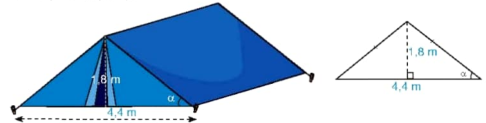
\includegraphics{images/9T4-OTC4.35}
	\end{center}
	\loigiai{
	Ta có $\cos \alpha=\dfrac{1{,}8}{2{,}2}=\dfrac{9}{1}\Rightarrow \alpha\approx 35^\circ5'$.
	}
\end{bt}
%%==========Bài 12
\begin{bt}
	Một cây cao bị gãy, ngọn cây đổ xuống mặt đắt. Ba điểm: gốc cây, điểm gãy, ngọn cây tạo thành một tam giác vuông. Đoạn cây gãy tạo với mặt đất góc $20^{\circ}$ và chắn ngang lối đi một đoạn $5 \mathrm{~m}$. Hỏi trước khi bị gẫy, cây cao khoảng bao nhiêu mét (làm tròn kết quả đến hàng phấn mười)?
	\begin{center}
	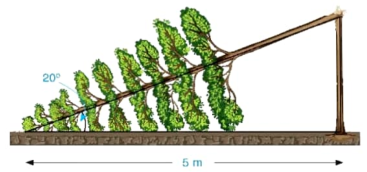
\includegraphics{images/9T4-OTC4.36}
	\end{center}
\loigiai{
	\immini{Xét tam giác $ABC$ vuông tại $A$ có $\widehat{C}=20^\circ$, $CA=5$ m.\\
	Khi đó chiều cao của cây trước khi gãy là $AB+BC$.\\
	Ta có $\tan C=\dfrac{AB}{CA}\Rightarrow AB=CA\cdot\tan C=5\cdot\tan 20^\circ\approx1{,}8$ m.\\
	$\cos C=\dfrac{CA}{BC}\Rightarrow BC=\dfrac{CA}{\cos C}=\dfrac{5}{\cos 20^\circ}\approx5{,}3$ m.\\
	Vậy chiều cao của cây là $AB+BC=1{,}8+5{,}3=7{,}1$ m.}{\begin{tikzpicture}[scale=1, font=\footnotesize, line join=round, line cap=round, >=stealth]
	\def\r{2}
	\path
	(0,0) coordinate (A)
	(0,2) coordinate (B)
	(-3.5,0) coordinate (C)
	;
	\draw
	(A)--(B)--(C)--(A)node[midway,below]{5 m}
	pic[draw, angle radius=2mm]{right angle=B--A--C};
	\foreach \x/\g in{A/-90, C/-90, B/0} \fill[black](\x) circle (1pt) ($(\x)+(\g:3mm)$) node{\x};
	\pic[draw, angle radius=3mm]{angle=A--C--B};
\end{tikzpicture}}
}
\end{bt}
%4.29. 
%4.30. 
%%==========Bài 13
\begin{bt}
	\immini{Hai điểm $P$ và $Q$ cách nhau $203$ m và thẳng hàng với chân của một toà tháp (Hình bên). Từ đỉnh của toà tháp đó, một người nhìn thấy hai điểm $P$, $Q$ với hai góc nghiêng xuống lần lượt là $38^\circ$ và $44^\circ$. Tính chiều cao của toà tháp (kết quả làm tròn đến hàng đơn vị của mét).}{\begin{tikzpicture}[line join=round, line cap=round,scale=0.6,transform shape]
	\definecolor{darkgray}{rgb}{0.66, 0.66, 0.66}
	\definecolor{arsenic}{rgb}{0.23, 0.27, 0.29}
	\def\N{ 
	(.5,-3)--(.5,-.5)--(.35,-.5)--(.35,1.3)--(.2,1.3)--(.2,2.8)--(.1,2.8)--(.1,3.7)--(-.1,3.7)--(-.1,2.4)--(-.2,2.4)--(-.2,1)--(-.4,1)--(-.4,-3)--cycle
	;
	}
	\path
	(0,3.7) coordinate (M)
	(0,-3) coordinate (N)
	($(N)+(180:1)$) coordinate (x)
	($(M)+(-136:1)$) coordinate (q)
	($(M)+(-142:1)$) coordinate (p)
	($(M)+(180:1)$) coordinate (y)
	(intersection of N--x and M--q) coordinate (Q)
	(intersection of N--x and M--p) coordinate (P)
	;
	\fill[darkgray] \N;
	\draw[pattern=horizontal lines, pattern color=gray]\N;
	\draw[pattern={vertical lines}, pattern color=gray]\N;
	\fill[arsenic!90] (.5,-2.2)--(-.4,-2.2)--(-.4,-2.1)--(.5,-2.1)--cycle
	(.5,-.5)--(-.4,-.5)--(-.4,-.65)--(.5,-.65)--cycle
	(.35,.8)--(-.4,.8)--(-.4,.9)--(.35,.9)--cycle
	(.2,2.2)--(-.2,2.2)--(-.2,2.1)--(.2,2.1)--cycle
	(.2,2.5)--(.2,2.8)--(.1,2.8)--(.1,3.7)--(-.1,3.7)--(-.1,2.5)--cycle
	;
	\draw (.4,-3)--(.4,-2.4)--(.5,-2.4)
	(-.3,-3)--(-.3,-2.5)--(-.4,-2.5)
	(.2,-3)--(.2,1.3) (0,-3)--(0,2.5) (-.1,-3)--(-.1,2.5) (-.2,-3)--(-.2,0)--(-.1,0);
	\draw (N)--(P)--(M)--(Q);
	\draw[red,line width=1pt,-latex] (N)--(M)--++(180:8)node[above]{$x$};
	\foreach \x/\g in {M/90,N/-90,P/-130,Q/-90}\fill[black](\x) circle (1pt) +(\g:3mm) node {$\x$};
	\pic[draw,angle radius=2mm]{angle=y--M--P};
	\pic[draw,angle radius=7mm,double]{angle=y--M--Q};
	\node at ($(M)+(-161:0.4)$){\tiny $38^\circ$};
	\node at ($(M)+(-158:0.9)$){\tiny $44^\circ$};
	\node[below] at ($(P)!0.5!(Q)$){\tiny $203$ m};
	\end{tikzpicture}}
	\loigiai{
	Đặt chiều cao của tháp là $h=MN$.\\
	Ta có $\widehat{NQM}=\widehat{QMx}=44^\circ$ (hai góc so le trong);\\
	$\widehat{NPM}=\widehat{PMx}=38^\circ$ (hai góc so le trong).\\
	Tam giác $MNQ$ vuông tại $N$ nên 
	$$\tan Q=\dfrac{MN}{QN}\Rightarrow QN=\dfrac{MN}{\tan Q}\Rightarrow QN=\dfrac{h}{\tan44^\circ}.$$
	Tam giác $NPM$ vuông tại $N$ nên 
	$$\tan P=\dfrac{MN}{PN}\Rightarrow PN=\dfrac{MN}{\tan P}\Rightarrow PN=\dfrac{h}{\tan 38^\circ}.$$
	Mà $QN=PN-203$ nên $\dfrac{h}{\tan44^\circ}=\dfrac{h}{\tan 38^\circ}-203$.\\
	Suy ra $\dfrac{h}{\tan 38^\circ}-\dfrac{h}{\tan44^\circ}=203\Rightarrow \dfrac{h}{0{,}244}=203\Rightarrow h=0{,}244\cdot203\approx50$ m.\\
	Vậy chiều cao của tháp gần $50$ m.
	}
\end{bt}
%%==========Bài 14
\begin{bt}
	\immini{Hai chiếc tàu thuỷ $B$ và $C$ cùng xuất phát từ một vị trí $A$, đi thẳng theo hướng tạo thành một góc $60^\circ$. Tàu $B$ chạy với tốc độ $20$ hải lí/giờ, tàu $C$ chạy với tốc độ $15$ hải lí/giờ. Hỏi sau $1{,}5$ giờ hai tàu $B$ và $C$ cách nhau bao nhiêu hải lí (kết quả làm tròn đến hàng phần trăm)?}{\begin{tikzpicture}[scale=0.8]
	\definecolor{maunuoc}{rgb}{2,126,188}
	\def\a{7};\def\b{5};
	\fill[cyan!80] (0,0)--(\a,0)--(\a,\b/2)--(\a/3,\b)--(0,\b)--cycle;
	\fill[pink!50!violet] (\a,\b/2)--(\a,\b*3/4)--(\a*2/3,\b)--(\a/3,\b)--cycle;
	\fill[gray] (\a,\b*3/4)--(\a,\b)--(\a*2/3,\b);
	\draw (0,0) rectangle (\a,\b);
	\draw[line width=1pt] ($(\a,\b/2)!0.6!(\a/3,\b)$)node[above right]{$A$}--++(-110:2)node[right]{$C$}
	($(\a,\b/2)!0.6!(\a/3,\b)$)--++(-170:3)node[above]{$B$};
	\node[rotate=70,left] at ($(\a,\b/2)!0.6!(\a/3,\b)+(-110:2)$){\twemoji[scale=1]{26f4}};
	\node[rotate=10,left] at ($(\a,\b/2)!0.6!(\a/3,\b)+(-170:3)$){\twemoji[scale=1]{26f4}};
	\node[rotate=-30,left,xscale=-1] at ($(\a,\b/2)!0.6!(\a/3,\b)+(-10:1)$){\twemoji[scale=0.4]{1f69a}};
	\node[rotate=-30,left,xscale=-1] at ($(\a,\b/2)!0.6!(\a/3,\b)+(-15:1.5)$){\twemoji[scale=0.4]{1f69b}};
	\node[rotate=-30,left] at ($(\a,\b/2)!0.6!(\a/3,\b)+(35:1.2)$){\twemoji[scale=0.4]{1f692}};
	\node[rotate=-30,left] at ($(\a,\b/2)!0.6!(\a/3,\b)+(15:1.5)$){\twemoji[scale=0.4]{1f699}};
	\node[rotate=-30,left] at ($(\a,\b/2)!0.6!(\a/3,\b)+(130:0.5)$){\twemoji[scale=0.4]{1f68f}};
	\node[rotate=-30,left] at ($(\a,\b/2)!0.6!(\a/3,\b)+(0:2.65)$){\twemoji[scale=0.4]{1f68f}};
	\node at ($(\a,\b/2)!0.6!(\a/3,\b)+(-140:0.5)$){$60^\circ$};
	\end{tikzpicture}}
	\loigiai{
	\immini{Sau $1{,}5$ giờ tàu $B$ đi được $1{,}5\cdot20=30$ hải lí và tàu $C$ đi được $1{,}5\cdot15=22{,}5$ hải lí.\\
	Gọi $CH$ là đường cao tam giác $ABC$. Tam giác $AHC$ vuông tại $H$ nên
	\begin{itemize}
	\item $HC=AC\sin A=22{,}5\cdot\sin 60^\circ=\dfrac{45\sqrt{3}}{4}$.
	\item $AH=AC\cos A=22{,}5\cdot\cos 60^\circ=\dfrac{45}{4}$.
	\end{itemize}
	}{\begin{tikzpicture}[scale=1, font=\footnotesize, line join=round, line cap=round, >=stealth]
	\path
	(0,0) coordinate (A)
	(1.5,3) coordinate (C)
	(4,0) coordinate (B)
	($(A)!(C)!(B)$) coordinate (H)
	;
	\draw 
	(A)--(B)node[midway,below]{$30$}--(C)--(A)node[midway,above left]{$22{,}5$}
	(C)--(H);
	\foreach \p/\g in {A/200, B/-15, C/90, H/-90}
	\draw[fill=black] (\p) circle (1pt) node[shift=(\g:3mm)] {$\p$};
	\pic["\tiny{$60$}",draw,angle radius=8mm]{angle=B--A--C};
	\end{tikzpicture}}
	\noindent Suy ra $HB=AB-AH=30-\dfrac{45}{4}=\dfrac{75}{4}$.\\
	Tam giác $CHB$ vuông tại $H$ nên theo định lí Pi-ta-go ta có
	$$BC^2=HC^2+HB^2=\left(\dfrac{45\sqrt{3}}{4}\right)^2+\left(\dfrac{75}{4}\right)^2=\dfrac{2925}{4}\Rightarrow BC\approx 27{,}04\text{ (hải lí).}$$	
	}
\end{bt}
%%=====Bài 2
%%==========Bài 15
\begin{bt}%[MaT-SGK9-Moi]%[Thầy Hải Toán - Quan Ón]
	\immini
	{
	Trong trò chơi xích đu ở Hình $41$, khi dây căng xích đu (không dãn) $OA=3 \mathrm{~m}$ tạo với phương thẳng đứng một góc là $\widehat{AOH}=43^{\circ}$ thì khoảng cách $AH$ từ em bé đến vị trí cân bằng là bao nhiêu mét (làm tròn kết quả đến hàng phần trăm)?
	}
	{
	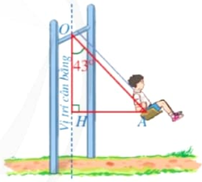
\includegraphics[scale=.75]{images/9C4-OTC-1}
	}
	\loigiai
	{
	Theo hình vẽ ta có khoảng cách từ em bé đến vị trí cân bằng là đoạn $AH$.\\
	Theo tỉ số lượng giác trong tam giác vuông $OAH$ vuông tại $H$ ta có \allowdisplaybreaks
	\begin{eqnarray*}
	&&\sin\widehat{HOA}=\dfrac{HA}{OA}\\
	&& HA=OA\cdot\sin\widehat{HOA}\\
	&& HA=3\cdot\sin 43^\circ\\
	&& HA\approx 2{,}05.
	\end{eqnarray*}	
	Vậy khoảng cách cần tìm là $AH\approx 2{,}05$ (m).
	}
\end{bt}
%%==========Bài 16
\begin{bt}%[MaT-SGK9-Moi]%[Quan Ón - Thầy Hải Toán]
	Một người đứng ở vị trí $B$ trên bờ sông muốn sử dụng la bàn để ước lượng khoảng cách từ vị trí đó đến một vị trí $A$ ở trên một cù lao giữa dòng sông.\\
	Người đó đã làm như sau
	\immini{
	\begin{itemize}
	\item Sử dụng la bàn, xác định được phương $BA$ lệch với phương Nam - Bắc về hướng Đông $52^\circ$.
	\item Người đó di chuyển đến vị trí $C$, cách $B$ một khoảng là $187$ m. Sử dụng la bàn, xác định được phương $CA$ lệch với phương Nam - Bắc về hướng Tây $27^\circ$; $CB$ lệch với phương Nam - Bắc về hướng Tây $70^\circ$ (Hình bên).
	\end{itemize}
	}{
	\begin{tikzpicture}[>=stealth,line join=round,line cap=round,font=\footnotesize,scale=1]
	\path 
	(5.26,2.44) coordinate (A)
	(3.48,1.02) coordinate (B)
	(7,0) coordinate (C)
	(3.48,3.6) coordinate (x)
	(7,4) coordinate (y)
	($(B)!(A)!(C)$) coordinate (H);
	\draw (A)--(B)--(C)--(A);
	\foreach \l/\g in {A/90,B/-135,C/-45}
	\draw[fill=black] (\l) circle (1pt) +(\g:.3) node{$\l$};
	\draw[<->] (0.46,1.98)--(1.54,1.98);
	\draw[<->] (0.98,2.5)--(0.98,1.5);
	\fill (0.46,1.98) node[left]{Tây};
	\fill (1.54,1.98) node[right]{Đông};
	\fill (0.98,2.5) node[above]{Bắc};
	\fill (0.98,1.5) node[below]{Nam};
	\end{tikzpicture}
	}
	\noindent
	Em hãy giúp người đó tính khoảng cách $AB$ từ những dữ liệu trên (làm tròn kết quả đến hàng đơn vị của mét).
	\loigiai{
	\begin{center}
	\begin{tikzpicture}[>=stealth,line join=round,line cap=round,font=\footnotesize,scale=1]
	\path 
	(5.26,2.44) coordinate (A)
	(3.48,1.02) coordinate (B)
	(7,0) coordinate (C)
	(3.48,3.6) coordinate (x)
	(7,4) coordinate (y)
	($(B)!(A)!(C)$) coordinate (H);
	\draw (A)--(B)--(C)--(A)--(H) (B)--(x) (C)--(y);
	\foreach \l/\g in {A/90,B/-135,C/-45,H/-90}
	\draw[fill=black] (\l) circle (1pt) +(\g:.3) node{$\l$};
	\fill (x) node[right]{$x$};
	\fill (y) node[right]{$y$};
	\pic[draw,angle radius=2mm,angle eccentricity=1.5] {right angle = A--H--C};
	\pic[draw,angle radius=4mm,angle eccentricity=1.5] {angle = A--B--x};
	\pic[draw,angle radius=4mm,angle eccentricity=1.5] {angle = y--C--A};
	\pic[draw,angle radius=5mm,angle eccentricity=1.5] {angle = y--C--A};
	\draw (B) circle (1pt) +(55:.65) node[scale=0.8]{$52^\circ$};
	\draw (C) circle (1pt) +(105:.75) node[scale=0.8]{$27^\circ$};
	\draw[<->] (0.46,1.98)--(1.54,1.98);
	\draw[<->] (0.98,2.5)--(0.98,1.5);
	\fill (0.46,1.98) node[left]{Tây};
	\fill (1.54,1.98) node[right]{Đông};
	\fill (0.98,2.5) node[above]{Bắc};
	\fill (0.98,1.5) node[below]{Nam};
	\end{tikzpicture}
	\end{center}
	Theo đề bài, ta có $\widehat{ABx} = 52^\circ$, $\widehat{ACy} = 27^\circ$, $\widehat{BCy} = 70^\circ$.\\
	Suy ra $\widehat{BCA} = \widehat{BCy} - \widehat{ACy} = 70^\circ - 27^\circ = 43^\circ$.\\
	Hơn nữa, vì $Bx \parallel Cy$ nên $\widehat{CBx} + \widehat{BCy} = 180^\circ \Rightarrow \widehat{CBx} = 180^\circ - \widehat{BCy} = 180^\circ - 70^\circ = 110^\circ$.\\
	Suy ra $\widehat{ABC} = \widehat{CBx} - \widehat{ABx} = 110^\circ - 52^\circ = 58^\circ$.\\
	Gọi $AH$ là đường cao của $\triangle ABC$.\\ 
	Xét $\triangle ABH$ vuông tại $H$, ta có
	$$ \tan \widehat{ABH} = \dfrac{AH}{BH} \Rightarrow BH = \dfrac{AH}{\tan\widehat{ABH}} = \dfrac{AH}{\tan 58^\circ}. $$
	Xét $\triangle ACH$ vuông tại $H$, ta có
	$$ \tan \widehat{ACH} = \dfrac{AH}{CH} \Rightarrow CH = \dfrac{AH}{\tan\widehat{ACH}} = \dfrac{AH}{\tan 43^\circ}. $$
	Mặt khác, ta có
	$$ BH + CH = BC \Rightarrow \dfrac{AH}{\tan 58^\circ} + \dfrac{AH}{\tan 43^\circ} = 187 \Rightarrow AH = \dfrac{187}{\dfrac{AH}{\tan 58^\circ} + \dfrac{AH}{\tan 43^\circ}} \approx 110 \textrm{ (m).} $$
	Xét $\triangle ABH$ vuông tại $H$, ta có
	$$ \sin\widehat{ABH} = \dfrac{AH}{AB} \Rightarrow AB = \dfrac{AH}{\sin\widehat{ABH}} = \dfrac{110}{\sin 58^\circ} \approx 130 \textrm{ (m).} $$
	Vậy khoảng cách $AB$ gần bằng $130$ mét.
	}
\end{bt}
%%==========Bài 17
\begin{bt}
	\immini{ĐỐ VUI. Chu vi Trái Đất bằng bao nhiêu?\\
	Vào khoảng năm 200 trước Công nguyên, Eratosthenes (O-ra-tô-xten), một nhà toán học và thiên văn học người Hy Lạp, đã ước lượng được \lq\lq chu vi\rq\rq~của Trái Đát (chu vi của đường Xích Đạo) nhờ hai quan sát sau:\\
	1. Hồi đó, hằng năm cứ vào trưa ngày Hạ chi (21/6), người ta thấy tia sáng mặt trời chiếu thẳng xuống đáy một cái giếng sâu nổi tiếng ỏ thành phố Syene (Xy-en), tức là tia sáng chiếu thẳng đứng.\\
	2. Cũng vào trưa một ngày Hạ chí, ở thành phố Alexandria (A-léch-xăng-đri-a) cách Syene $800 \mathrm{~km}$, Eratosthenes thấy một tháp cao $25 \mathrm{~m}$ có bóng trên mặt đất dài $3{,}1 \mathrm{~m}$.}{
	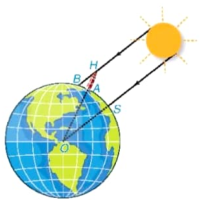
\includegraphics[width=4.5cm]{images/9T4-OTC4.38}}
	\noindent Từ hai quan sát trên, ông có thể tính xấp xỉ \lq\lq chu vi\rq\rq~của Trái Đất như thế nào? (trên hình, điểm $O$ là tâm Trái Đất, điểm $S$ tuợng trung cho thành phố Syene, điểm $A$ tượng trưng cho thành phớ Alexandria, điểm $H$ là đỉnh của tháp, bóng của tháp trên mặt đất được coi là đoạn thẳng $A B$).
	\loigiai{
	\immini{Gọi $c$ là chu Trái đất, góc $\widehat{AOS}=\alpha$.\\
	Ta có $c=AS\cdot \dfrac{360^\circ}{\alpha}=800\cdot\dfrac{360^\circ}{\alpha}$.\\
	Vì các tia nắng chiếu thẳng đứng nên $BH\parallel SO$ do đó $\widehat{AOS}=\widehat{AHB}$ (so le trong).\\
	Trong tam giác $ABH$ vuông tại $A$ có $$\tan H=\dfrac{AB}{AH}=\dfrac{3{,}1}{25}\approx0{,}124\Rightarrow \widehat{H}\approx 7{,}07^\circ.$$
	Vì $\widehat{AOS}=\widehat{AHB}$ nên $\alpha=7{,}07^\circ$.\\
	Vậy chu vi Trái đất là $c=800\cdot\dfrac{360^\circ}{7{,}07^\circ}\approx 70736$ $\mathrm{(km)}$.}{\begin{tikzpicture}[scale=1, font=\footnotesize, line join=round, line cap=round, >=stealth]
	\def\r{2}
	\path
	(0,0) coordinate (A)
	(-0.5,0) coordinate (B)
	(0,1) coordinate (H)
	($(B)!4!(A)$) coordinate (S)
	($(H)!4!(A)$) coordinate (O)
	;
	\draw
	(B)--(S)--(O)--(H)--cycle
	pic[draw, angle radius=2mm]{right angle=B--A--H};
	\foreach \x/\g in{A/45, S/0, B/180, O/-10, H/30} \fill[black](\x) circle (1pt) ($(\x)+(\g:3mm)$) node{\x};
	\end{tikzpicture}}
	}
\end{bt}
%%==========Bài 18
\begin{bt}
	Cho hình thang $ABCD$ ($AB\parallel CD$), $\widehat{C} = 36^{\circ}$; $\widehat{D} = 50^{\circ}$. Biết $AB = 4\, \mathrm{cm}$, $AD = 6\, \mathrm{cm}$. Tính chu vi hình thang.
	\loigiai
	{\immini
	{Vẽ $AH\perp CD$ và $BK\perp CD$, dễ thấy $AHKB$ là hình chữ nhật.\\
	Do đó $AH = BK$ và $AB = HK$.\\
	Xét $\triangle ADH$ vuông tại $H$, ta có\\
	$DH = AD\cdot\cos\widehat{ADH} = 6\cdot \cos 50^{\circ}\approx 4{,}6\, \left(\mathrm{cm}\right)$.\\
	Tương tự, xét $\triangle BKC$ vuông tại $K$, ta có $KC = BK\cdot\cot\widehat{BCK} = 4{,}6\cdot \cot 36^{\circ}\approx 6{,}3\, \left(\mathrm{cm}\right)$\\
	và $BC = \dfrac{BK}{\sin\widehat{KCB}} = \dfrac{4{,}6}{\sin 36^{\circ}}\approx 7{,}8\, \left(\mathrm{cm}\right)$.\\
	Ta có $DC = DH + HK + KC = 3{,}9 + 4 + 6{,}3\approx 14{,}2\, \left(\mathrm{cm}\right)$.\\
	Do đó chu vi của hình thang là $4 + 7{,}8 + 14{,}2 + 6 14{,}2\approx 32\, \left(\mathrm{cm}\right)$. 	
	}
	{\begin{tikzpicture}[line join = round, line cap = round,>=stealth,
	font=\footnotesize,scale=.8]
	\tkzDefPoints{0/0/D}
	\coordinate (C) at ($(D)+(9,0)$);
	\tkzDefShiftPoint[D](50:3){A}
	\coordinate (B) at ($(A)+(3,0)$);
	\tkzDefPointBy[projection= onto C--D](A)
	\tkzGetPoint{H}
	\tkzDefPointBy[projection= onto C--D](B)
	\tkzGetPoint{K}
	\pgfresetboundingbox
	\tkzDrawPolygon(A,B,C,D)
	\tkzDrawSegments(A,H B,K)
	\tkzDrawPoints[fill=black](D,C,A,B,H,K)
	\tkzLabelAngles[pos=-.8](A,D,H){$50^\circ$}
	\tkzLabelAngles[pos=1.2](B,C,K){$36^\circ$}
	\path (B)--(A) node[above left,midway]{$4$};
	\path (A)--(D) node[above left,midway]{$6$};
	\tkzLabelPoints[above](A,B)
	\tkzLabelPoints[left](D)
	\tkzLabelPoints[right](C)
	\tkzLabelPoints[below](H,K)
	\end{tikzpicture}
	}	
	}
\end{bt}
%%==========Bài 19
\begin{bt}
	Cho hình thang cân $ABCD$ ($AB\parallel CD$). Biết $AD = 2{,}1\, \mathrm{cm}$; $CD = 6{,}0\, \mathrm{cm}$ và $\widehat{D} = 48^{\circ}$.
	\begin{listEX}[2]
	\item Tính độ dài $AB$.
	\item Tính diện tích hình thang $ABCD$. 
	\end{listEX}
	\loigiai
	{\begin{enumerate}
	\item Kẻ các đường cao $AH\perp CD$ và $BK\perp CD$. 
	\immini
	{Dễ thấy $ABKH$ là hình chữ nhật nên $AB = HK$.\\
	Xét $\triangle AHD$ và $\triangle BKC$, do giả thiết suy ra $AD = BC$ và $\widehat{ADH} = \widehat{BCK}$
	nên $\triangle AHD = \triangle BKC$.\\
	Do đó $DH = KC$ và $HK = DC - 2DH$.	\\
	Xét tam giác vuông $AHD$ ta có $DH = AB\cdot\cos\widehat{ADH} = 2{,}1\cdot \cos 48^{\circ}\approx 1{,}4\, \left(\mathrm{cm}\right)$.\\
	Suy ra $AB = 6{,}0 - 2\cdot 1{,}4 \approx 3{,}2\, \left(\mathrm{cm}\right)$.
	}
	{\begin{tikzpicture}[line join = round, line cap = round,>=stealth,
	font=\footnotesize,scale=.9]
	\tkzDefPoints{0/0/D}
	\coordinate (C) at ($(D)+(7,0)$);
	\tkzDefShiftPoint[D](50:3){A}
	\coordinate (B) at ($(A)+(3,0)$);
	\tkzDefPointBy[projection= onto C--D](A)
	\tkzGetPoint{H}
	\tkzDefPointBy[projection= onto C--D](B)
	\tkzGetPoint{K}
	\pgfresetboundingbox
	\tkzDrawPolygon(A,B,C,D)
	\tkzDrawSegments(A,H B,K)
	\tkzDrawPoints[fill=black](D,C,A,B,H,K)
	\tkzLabelAngles[pos=-.8](A,D,H){$48^\circ$}
	\tkzLabelAngles[pos=.8](B,C,K){$48^\circ$}
	\path (C)--(D) node[below, midway]{$6$};
	\path (A)--(D) node[above left,midway]{$2{,}1$};
	\tkzLabelPoints[above](A,B)
	\tkzLabelPoints[left](D)
	\tkzLabelPoints[right](C)
	\tkzLabelPoints[below](H,K)
	\tkzMarkRightAngles(A,H,K B,K,H)
	\end{tikzpicture}
	}	 
	\item Gọi $S$ là diện tích hình thang $ABCD$. Khi đó $S = \dfrac{\left(AB + CD\right)\cdot AH}{2}$.\\
	Xét tam giác vuông $ADH$ ta có $AH = AB\cdot\sin\widehat{ADH} = 2{,}1\cdot \sin 48^{\circ}\approx 1{,}56\, \left(\mathrm{cm}\right)$.\\
	Nên $S = \dfrac{\left(3{,}2 + 6{,}0\right)\cdot 1{,}56}{2}\approx 7{,}88\, \left(\mathrm{cm}^2\right)$. 
	\end{enumerate}
	}
\end{bt}
%%%%%%%%%%%%
\subsection{Bài tập trắc nghiệm}
\Opensolutionfile{ans}[ans/ans-9T4-OTC]
%%==========Câu 1
\begin{ex}
	\immini{Trong hình bên, $\cos \alpha$ bằng
	\choice
	{$\dfrac{5}{3}$}
	{$\dfrac{3}{4}$}
	{\True $\dfrac{3}{5}$}
	{$\dfrac{4}{5}$}}{\begin{tikzpicture}[scale=1, font=\footnotesize, line join=round, line cap=round, >=stealth]
	\def\r{2}
	\path
	(130:\r) coordinate (A)
	(180:\r) coordinate (B)
	(0:\r) coordinate (C)
	;
	\draw
	($(B)+(0.4,0.3)$)node {$\alpha$}
	(A)--(B)node[midway,left]{$3$}--(C)node[midway,below]{$5$}--(A)node[midway,above]{$4$}
	pic[draw, angle radius=2mm]{right angle=B--A--C};
	\pic[draw, angle radius=3mm]{angle=C--B--A};
	\end{tikzpicture}}
	\loigiai{
	Ta có $\cos\alpha=\dfrac{3}{5}$.
	}
\end{ex}
%%==========Câu 2
\begin{ex}
	\immini{Trong tam giác $M N P$ vuông tại $M$, $\sin \widehat{M N P}$ bằng
	\choice
	{$\dfrac{P N}{N M}$}
	{\True $\dfrac{M P}{P N}$}
	{$\dfrac{M N}{P N}$}
	{$\dfrac{M N}{M P}$}}{\begin{tikzpicture}[scale=0.85, font=\footnotesize, line join=round, line cap=round, >=stealth]
	\def\r{2}
	\path
	(0,0) coordinate (M)
	(0,2) coordinate (N)
	(3.5,0) coordinate (P)
	;
	\draw
	(M)--(N)--(P)--cycle
	pic[draw, angle radius=2mm]{right angle=N--M--P};
	\foreach \x/\g in{M/-150, N/180, P/0} \fill[black](\x) circle (1pt) ($(\x)+(\g:3mm)$) node{\x};
	\pic[draw, angle radius=3mm]{angle=M--N--P};
	\end{tikzpicture}}
	\loigiai{
	$\sin \widehat{M N P}=\dfrac{MP}{PN}$.
	}
\end{ex}
%%==========Câu 3
\begin{ex}
	\immini{Trong tam giác $A B C$ vuông tại $A$, $\tan B$ bằng
	\choice
	{$\dfrac{A B}{A C}$}
	{\True $\dfrac{A C}{A B}$}
	{$\dfrac{A B}{B C}$}
	{$\dfrac{B C}{A C}$}}{\begin{tikzpicture}[scale=0.85, font=\footnotesize, line join=round, line cap=round, >=stealth]
	\def\r{2}
	\path
	(0,0) coordinate (A)
	(0,2) coordinate (C)
	(-3.5,0) coordinate (B)
	;
	\draw
	(A)--(B)--(C)--cycle
	pic[draw, angle radius=2mm]{right angle=B--A--C};
	\foreach \x/\g in{A/-90, B/-90, C/0} \fill[black](\x) circle (1pt) ($(\x)+(\g:3mm)$) node{\x};
	\pic[draw, angle radius=3mm]{angle=A--B--C};
	\end{tikzpicture}}
	\loigiai{
	Ta có $\tan B=\dfrac{AC}{AB}$,
	}
\end{ex}
%%==========Câu 4
\begin{ex}
	\immini{Cho hình bên. Độ dài cạnh $BC$ là
	\choice
	{$4$ cm}
	{$8\sqrt{3}$ cm}
	{$\dfrac{8\sqrt{3}}{3}$ cm}
	{\True $16$ cm}}{\begin{tikzpicture}[scale=0.85, font=\footnotesize, line join=round, line cap=round, >=stealth]
	\path
	(0,0) coordinate (A)
	(0,2) coordinate (B)
	(4,0) coordinate (C)
	;
	\draw 
	(A)--(B)node[midway,left]{$8\mathrm{~cm}$}--(C)--(A)
	;
	\foreach \p/\g in {A/200, B/150, C/0}
	\draw[fill=black] (\p) circle (1pt) node[shift=(\g:3mm)] {$\p$};
	\pic["\tiny{$30$}",draw,angle radius=10mm]{angle=B--C--A};
	\end{tikzpicture}}
	\loigiai{
	Tam giác $ABC$ vuông tại $A$ nên $\sin C=\dfrac{AB}{BC}\Rightarrow BC=\dfrac{AB}{\sin C}=\dfrac{8}{\sin30^{\circ}}=16$ cm.
	}
\end{ex}
%%==========Câu 5
\begin{ex}
	Với mọi góc nhọn $\alpha$, ta có
	\choice
	{\True $\sin \left(90^{\circ}-\alpha\right)=\cos \alpha$}
	{$\tan \left(90^{\circ}-\alpha\right)=\cos \alpha$}
	{$\cot \left(90^{\circ}-\alpha\right)=1-\tan \alpha$}
	{$\cot \left(90^{\circ}-\alpha\right)=\sin \alpha$}
	\loigiai{
	Ta có $\sin \left(90^{\circ}-\alpha\right)=\cos \alpha$.
	}
\end{ex}
%%==========Câu 6
\begin{ex}
	Giá trị $\tan 30^{\circ}$ bằng
	\choice
	{$\sqrt{3}$}
	{$\dfrac{\sqrt{3}}{2}$}
	{\True $\dfrac{1}{\sqrt{3}}$}
	{$1$}
	\loigiai{
	$\tan 30^{\circ}=\dfrac{1}{\sqrt{3}}$.
	}
\end{ex}
%%==========Câu 7
\begin{ex}
	Cho tam giác $ABC$ vuông tại $A$ có $AC=10$ cm, $\widehat{C}=60^\circ$. Độ dài hai cạnh còn lại là
	\choice
	{$AB=\dfrac{5\sqrt{3}}{3}$ cm; $BC=\dfrac{20\sqrt{3}}{3}$ cm}
	{$AB=\dfrac{5\sqrt{3}}{3}$ cm; $BC=\dfrac{14\sqrt{3}}{3}$ cm}
	{\True $AB=10\sqrt{3}$ cm; $BC=20$ cm}
	{$AB=\dfrac{10\sqrt{3}}{3}$ cm; $BC=\dfrac{20\sqrt{3}}{3}$ cm}
	\loigiai{
	\immini{Ta có 
	\begin{itemize}
	\item $\tan C=\dfrac{AB}{AC}\Rightarrow AB=AC\cdot \tan C=10\cdot\tan60^\circ=10\sqrt{3}$.
	\item $\cos C=\dfrac{AC}{BC}\Rightarrow BC=\dfrac{AC}{\cos C}=\dfrac{10}{\cos 60^\circ}=20$ cm.
	\end{itemize}}{\begin{tikzpicture}[scale=1, font=\footnotesize, line join=round, line cap=round, >=stealth]
	\path
	(0,0) coordinate (A)
	(0,2) coordinate (B)
	(4,0) coordinate (C)
	;
	\draw 
	(A)--(B)--(C)--(A)node[midway,below]{$10$}
	;
	\foreach \p/\g in {A/200, B/150, C/0}
	\draw[fill=black] (\p) circle (1pt) node[shift=(\g:3mm)] {$\p$};
	\pic["\tiny{$60$}",draw,angle radius=10mm]{angle=B--C--A};
	\end{tikzpicture}}
	}
\end{ex}
%%==========Câu 8
\begin{ex}
	Cho tam giác $ABC$ vuông tại $A$ có $BC=8$ cm, $AC=6$ cm. Tỉ số lượng giác $\tan C$ (kết quả làm tròn đến hàng phần trăm) là
	\choice
	{$0{,}87$}
	{$0{,}86$}
	{\True $0{,}88$}
	{$0{,}89$}
	\loigiai{
	Tam giác $ABC$ vuông tại $A$ nên $$BC^2=AC^2+AB^2\Rightarrow AB=\sqrt{BC^2-AC^2}=\sqrt{8^2-6^2}=2\sqrt{7}.$$
	Suy ra $\tan C=\dfrac{AB}{AC}=\dfrac{2\sqrt{7}}{6}\approx0{,}88$.
	}
\end{ex}
%%==========Câu 9
\begin{ex}
	Giá trị của biểu thức $B=\tan 20^\circ\cdot\tan 30^\circ\cdot \tan 40^\circ\cdot\tan 50^\circ\cdot \tan 60^\circ\cdot\tan 70^\circ$ là
	\choice
	{$2$}
	{\True $1$}
	{$3$}
	{$4$}
	\loigiai{
	Ta có $\begin{aligned}[t]B&=\tan 20^\circ\cdot\tan 30^\circ\cdot \tan 40^\circ\cdot\tan 50^\circ\cdot \tan 60^\circ\cdot\tan 70^\circ\\
	&=\cot 70^\circ\cdot \cot 60^\circ\cdot \cot 50^\circ\cdot \tan 50^\circ \cdot\tan 60^\circ\cdot\tan 70^\circ\\
	&=\left(\cot 70^\circ\cdot\tan 70^\circ\right) \left(\cot 60^\circ\cdot\tan 60^\circ\right) \left(\cot 50^\circ\cdot \tan 50^\circ\right)\\
	&=1.
	\end{aligned}$
	}
\end{ex}
%%==========Câu 10
\begin{ex}
	\immini{Một người quan sát ngọn hải đăng ở vị trí cao $149$ m so với mặt nước biển thì thấy một du thuyền ở xa với góc nghiêng xuống là $27^\circ$ (Hình 1). Hỏi thuyền cách xa chân hải đăng bao nhiêu mét (kết quả làm tròn đến hàng đơn vị)?
	\choice
	{\True $292$ m}
	{$288$ m}
	{$312$ m}
	{$151$ m}}{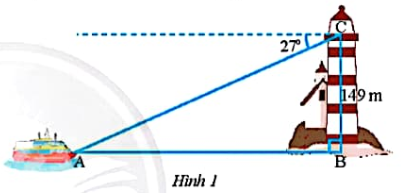
\includegraphics{images/9S4-OTC-hinh1.png}}
	\loigiai{
	Ta có $\widehat{CAB}=27^\circ$.\\
	Tam giác $ABC$ vuông tại $B$ nên $\tan A=\dfrac{BC}{AB}\Rightarrow AB=\dfrac{BC}{\tan A}=\dfrac{149}{\tan 27^\circ}\approx 292$ m.
	}
\end{ex}
%%==========Câu 11
\begin{ex}
	Cho tam giác $MNP$ có $\widehat{N}=70^\circ$, $\widehat{P}=38^\circ$, đường cao $MI=11{,}5$ cm. Độ dài cạnh $NP$ của tam giác $MNP$ (kết quả làm tròn đến hàng phần mười) bằng
	\choice
	{$20{,}9$ cm}
	{\True $18{,}9$ cm}
	{$40{,}6$ cm}
	{$16{,}9$ cm}
	\loigiai{
	\immini{
	Tam giác $NMI$ vuông tại $I$ nên\\ $\tan N=\dfrac{MI}{NI}\Rightarrow NI=\dfrac{MI}{\tan N}=\dfrac{11{,}5}{\tan 70^\circ}\approx4{,}2$ cm.\\
	Tam giác $PMI$ vuông tại $I$ nên\\ $\tan P=\dfrac{MI}{PI}\Rightarrow PI=\dfrac{MI}{\tan P}=\dfrac{11{,}5}{\tan 38^\circ}\approx14{,}7$ cm.\\
	Suy ra $NP=NI+IP=4{,}2+14{,}7=18{,}9$ cm.
	}{\begin{tikzpicture}[scale=0.85, font=\footnotesize, line join=round, line cap=round, >=stealth]
	\path
	(0,0) coordinate (N)
	(1,2) coordinate (M)
	(4,0) coordinate (P)
	($(N)!(M)!(P)$) coordinate (I)
	;
	\draw 
	(M)--(N)--(P)--cycle (M)--(I)
	;
	\foreach \p/\g in {M/90, N/180, P/0, I/-90}
	\draw[fill=black] (\p) circle (1pt) node[shift=(\g:3mm)] {$\p$};
	%	\pic["\tiny{$60$}",draw,angle radius=10mm]{angle=B--C--A};
	\end{tikzpicture}}
	}
\end{ex}
%%==========Câu 12
\begin{ex}
	Một cái thang dài $3$ m đặt sát bờ tường, biết góc tạo bởi thang và bờ thang là $40^\circ$. Hỏi chân thang đặt ở vị trí cách tường bao nhiêu mét (kết quả làm tròn đến hàng phần mười)?
	\choice
	{$1{,}9$ m}
	{\True $2{,}3$ m}
	{$1{,}8$ m}
	{$2{,}5$ m}
	\loigiai{
	\immini{
	Chân thang đặt ở vị trí cách tường là $AC$.\\
	Ta có $\cos A=\dfrac{AC}{AB}\Rightarrow AC=AB\cos A=3\cos40^{\circ}\approx 2{,}3$ m.
	}{\begin{tikzpicture}[scale=0.85, font=\footnotesize, line join=round, line cap=round, >=stealth]
	\path
	(0,0) coordinate (A)
	(3.5,3) coordinate (B)
	(3.5,0) coordinate (C)
	;
	\draw 
	(A)--(B)node[midway,left]{$3\mathrm{~m}$}--(C)--(A)
	;
	\foreach \p/\g in {A/200, B/90, C/0}
	\draw[fill=black] (\p) circle (1pt) node[shift=(\g:3mm)] {$\p$};
	\pic[draw,angle radius=2mm]{right angle=B--C--A};
	\pic["\tiny{$40$}",draw,angle radius=8mm]{angle=C--A--B};
	\end{tikzpicture}}
	}
\end{ex}
%%==========Câu 13
\begin{ex}
	Một chiếc máy bay lên với tốc độ $450$ km/h. Đường bay lên tạo với phương nằm ngang một góc $30^\circ$. Hỏi sau $3$ phút kể từ lúc cất cánh, máy bay cách mặt đât bao nhiêu kilômét theo phương thẳng đứng?
	\choice
	{$10{,}5$ km}
	{$12{,}75$ km}
	{$12$ km}
	{\True $11{,}25$ km}
	\loigiai{
	\immini{
	Sau $3$ phút máy bay bay được quãng đường là $$AB=450\cdot \dfrac{3}{60}=22{,}5\mathrm{~ km}.$$
	Ta có $$\sin A=\dfrac{BC}{AB}\Rightarrow BC=AB\sin A=22{,}5\cdot\sin 30^{\circ}=11{,}25\mathrm{~ km}.$$
	Vậy sau $3$ phút, máy bay cách mặt đất theo phương thẳng đứng $11{,}25$ km.
	}{\begin{tikzpicture}[scale=0.85, font=\footnotesize, line join=round, line cap=round, >=stealth]
	\path
	(0,0) coordinate (A)
	(4,3) coordinate (B)
	(4,0) coordinate (C)
	;
	\draw 
	(A)--(B)--(C)--(A)
	;
	\foreach \p/\g in {A/200, B/90, C/0}
	\draw[fill=black] (\p) circle (1pt) node[shift=(\g:3mm)] {$\p$};
	\pic[draw,angle radius=2mm]{right angle=B--C--A};
	\pic["\tiny{$30$}",draw,angle radius=8mm]{angle=C--A--B};
	\end{tikzpicture}}
	}
\end{ex}
\Closesolutionfile{ans}